\section{Experiments}
\label{sec:experiments}

% \sm{LinUCB imitation ReLU}

% \sm{TS K-arm, Bernoulli}


In this section, we perform preliminary simulations to demonstrate the ICRL capabilities of transformers and validate our theoretical findings. We remark that while similar experiments have been conducted in existing works~\citep{laskin2022context,lee2023supervised}, our setting differs in several aspects such as imitating the entire interaction trajectory in our pretrain loss~\eqref{eq:general_mle} as opposed to on the last (query) state only as in~\citet{lee2023supervised}. The code is available at~\href{https://github.com/licong-lin/in-context-rl}{https://github.com/licong-lin/in-context-rl}.


% as we train the transformer to imitate the whole interaction trajectory.\lc{not precise?}


We compare pretrained transformers against empirical average, LinUCB (or UCB), and Thompson sampling. We use a GPT-2 model~\cite{garg2022can,lee2023supervised} with $L = 8$ layers, $M=4$ heads, and embedding dimension $D=32$. We utilize ReLU attention layers, aligning with our theoretical construction. We pretrain the transformer with two setups: (1) Both context algorithm $\sAlg_0$ and expert algorithm $\sAlg_{\shortexp}$ use LinUCB (the Algorithm Distillation approach); (2) Context algorithms $\sAlg_0$ mixes uniform policy and Thompson sampling, while expert $\sAlg_{\shortexp} = \action_t^*$ provides optimal actions (DPT). See Appendix \ref{sec:exp_details} for further experimental details. 

% In this section, we investigate the performance of ICRL empirically on  stochastic linear bandit problems, and compare it with other online bandit algorithms including empirical average,  LinUCB (or UCB)  and Thompson sampling. We refer the reader to Appendix~\ref{sec:exp_details} for more details. In the experiments,  we use an $8$-layer transformer GPT-2 model with ReLU attention layers and pretrain the model with two different choices of context and expert algorithms. Namely, we consider (1). the context algorithm $\sAlg_{0}$ and the expert algorithm $\sAlg_{\shortexp}$  both to be LinUCB (i.e., Algorithm distillation). (2). The context algorithm $\sAlg_{0}$ is a mixture of the uniform policy and Thompson sampling, while  the expert  gives the optimal action $\sAlg_{\shortexp}=\action_t^*$  (i.e., the DPT approach). 

In the first setup, we consider stochastic linear bandits with $d=5$ and $A=10$. At each $t \in [200]$, the agent chooses an action $\action_t$ and receives reward $\reward_t=\<\action_t,\bw^*\>+\eps_t$ where $\eps_t\sim\cN(0,1.5^2)$. The parameter $\bw^*$ is from ${\rm Unif}([0,1]^d)$. The action set $\sA_t=\sA$ is fixed over time with actions i.i.d. from ${\rm Unif}([-1, 1]^d)$. We generate 100K trajectories using $\sAlg_0=\sAlg_{\shortexp}=\LinUCB$ and train transformer $\TF_\EstPar(\cdot)$ via Eq.~\eqref{eq:general_mle}. Figure~\ref{fig:regret_1} (left) shows regrets of the transformer (TF), empirical average (Emp), LinUCB, and Thompson sampling (TS). The transformer outperforms Thompson sampling and empirical average, and is comparable to LinUCB, agreeing with Theorem~\ref{thm:smooth_linucb}. The small regret gap between TF and LinUCB may stem from the limited capacity of the GPT2 model.


% For the first case, we consider a stochastic linear bandit with $d=5,A=10$.  We choose the time step $\totlen=200$. At each time $t\in[\totlen]$, the agent deploys an action $\action_t$ and the environment generates the reward $\reward_t=\<\action_t,\bw^*\>+\eps_t$, where the noise $\eps_t\sim\cN(0,\sigma^2)$ and $\sigma=1.5$.  We assume the true parameter $\bw^*$ is generated from the uniform distribution on $[0,1]^d$. Moreover, we assume the action set $\sA_t=\sA$ is fixed across time and the actions are i.i.d. samples from the uniform distribution on $[-1,1]^d$.  We generate $100000$ interaction trajectories with $\sAlg_0=\sAlg_{\shortexp}=\LinUCB$ and find the transformer $\TF_\EstPar(\cdot)$ via solving Eq.~\eqref{eq:general_mle}. We see in Figure~\ref{fig:regret_1} (left) that the transformer outperforms Thompson sampling and empirical average and is close to  LinUCB  in terms of regret. This aligns with our theoretical findings in Theorem~\ref{thm:smooth_linucb}. Moreover, we conjecture that the minor gap between TF and LinUCB is likely due to the limited expressivity of our small transformer model.


In the second setup, we consider multi-armed Bernoulli bandits with $d = 5$. The parameter $\bw^*$ is from ${\rm Unif}([0,1]^d)$. The fixed action set $\sA_t=\sA$ contains one-hot vectors $\{\be_i\}_{i=1}^d$ (multi-armed bandits). At each $t \in [200]$, the agent selects $\action_t$ receives reward $r_t \sim {\rm Bern}(\<\action_t,\bw^*\>)$. Let $\sAlg_{\mathrm{unif}}$ be the uniform policy. We use $\sAlg_{\mathrm{unif}}$ and $\sAlg_\TS$ as context algorithms to generate $50$K trajectories each. The expert is fixed as $\sAlg_\shortexp=\action^*$. We train transformer $\TF_\EstPar(\cdot)$ via Eq.~\eqref{eq:general_mle}. Figure~\ref{fig:regret_1} (right) shows regrets for the pretrained transformer (TF), empirical average (Emp), UCB, and Thompson sampling (TS).  The transformer aligns with Thompson sampling, validating Theorem~\ref{thm:ts_linear_regret}. However, TS underperforms UCB for Bernoulli bandits, as shown. 

% For the second case, we study a multi-armed Bernoulli bandit problem with $d=5$ and time step $\totlen=200$. We assume the true parameter $\bw^*$ is also generated following the uniform distribution on $[0,1]^d$ and the action set $\sA_t=\sA$  consists of the one-hot vectors $\{\be_i\}_{i=1}^d$.  At each time $t\in[\totlen]$, the agent selects an action $\action_t$ and the environment generates a reward $r_t$ from $\mathrm{Bern}(\<\action_t,\bw^*\>)$. Let $\sAlg_{\mathrm{unif}}$ denote the policy that  uniformly chooses  an action $\action_t$ at each time step. For both $\sAlg_\TS$ and $\sAlg_{\mathrm{unif}}$, we utilize them as the context algorithms and $\sAlg_\shortexp=\action_t^*$ as the expert to produce $50000$ i.i.d. interaction trajectories. These datasets are then merged to form one with $\sAlg_0=[\sAlg_{\TS}+\sAlg_{\mathrm{unif}}]/2$ and $\sAlg_\shortexp=\action_t^*$. We find $\TF_{\EstPar}$ via solving Eq.~\eqref{eq:general_mle} and the result is displayed in Figure~\ref{fig:regret_1}~(right). We observe that the regret of transformer is aligned with that of Thompson sampling, validating our finding in Theorem~\ref{thm:ts_linear_regret}. Moreover, it should be noted that TS is sub-optimal in Figure~\ref{fig:regret_1}~(right) since we only consider a small number of time steps.




\begin{figure}[t]
\centering  % Center the figure
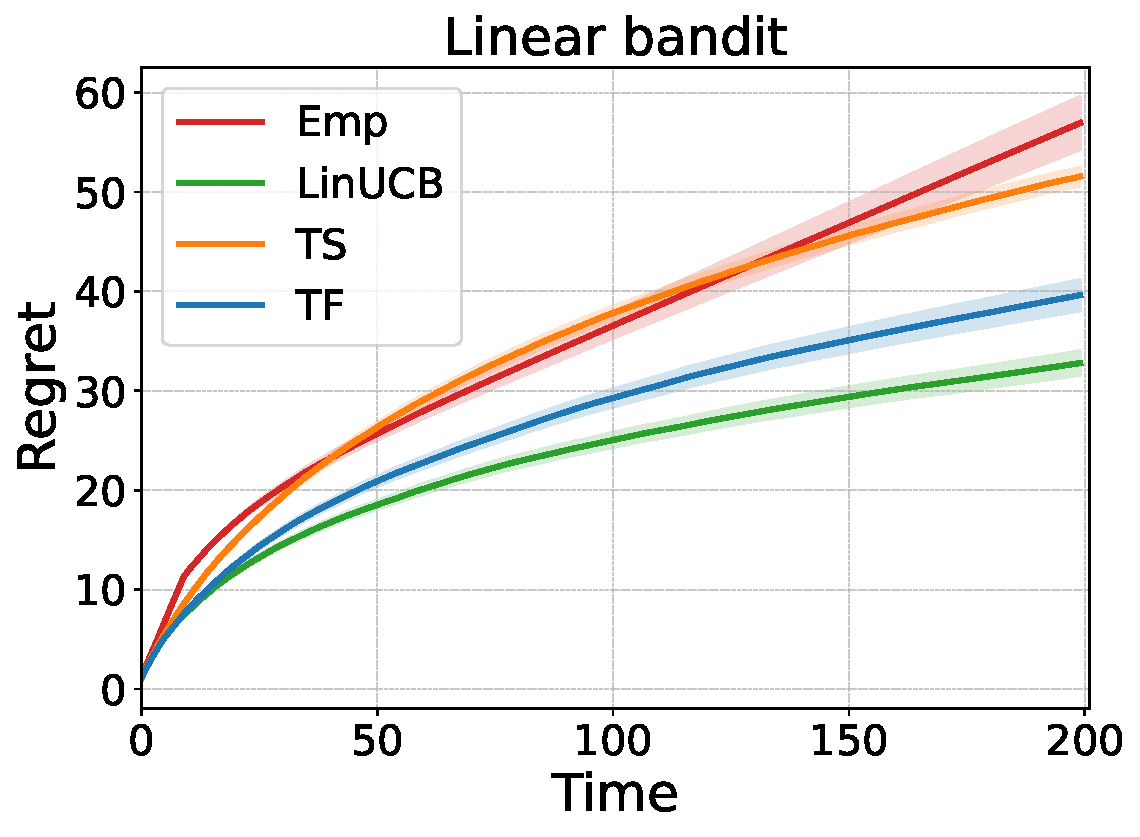
\includegraphics[width=0.35\linewidth]{Sections/figs/record_2_cum_True.pdf}
\hspace{2em}
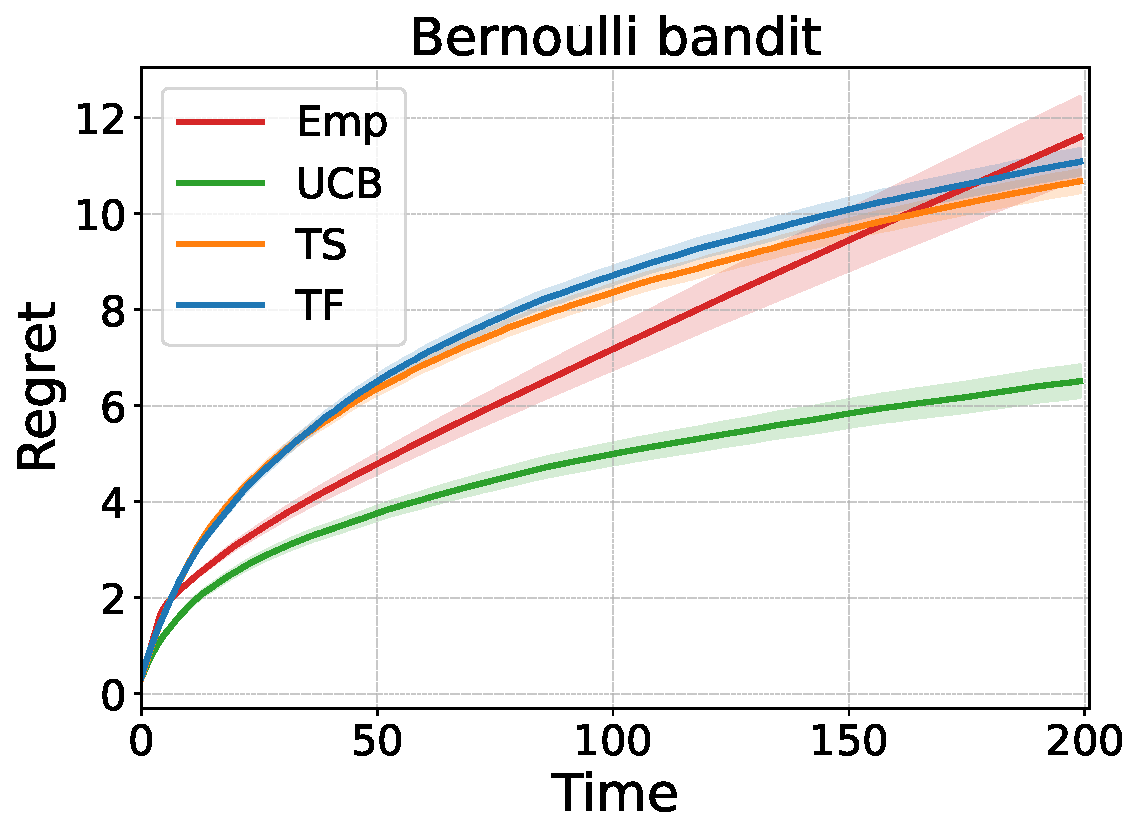
\includegraphics[width=0.35\linewidth]{Sections/figs/record_1_cum_True.pdf}
\vspace{-1em}
\caption{Regrets of transformer (TF), empirical average (Emp), Thompson sampling (TS) and LinUCB or UCB (LinUCB reduces to UCB for Bernoulli bandits). Left: linear bandit with $d=5$, $A=10$, $\sigma=1.5$, $\sAlg_0=\sAlg_\shortexp=\LinUCB$. Right: Bernoulli bandit with $d=5$, $\sAlg_0=(\sAlg_{\mathrm{unif}}+\sAlg_{\TS})/2$ and $\sAlg_\shortexp=\action^*$. The simulation is repeated 500 times. Shading displays the standard deviation of the regret estimates. } 
\label{fig:regret_1} 
\end{figure}

